% Generated from markdown/02.introduction.md; edit the Markdown source.
\section{Introduction}

\label{sec:introduction}

LLM-based query expansion in hybrid retrieval is commonly evaluated by fusing fixed top-\(L\) prefixes from dense and sparse rankings \citep{gao-etal-2023-precise, wang-etal-2023-query2doc, zhang-etal-2024-exploring-best, liu-zhang-2025-exp4fuse}. Yet \(L\) controls both ranking access and which cross-channel contributions enter fusion, so changing it may change the fused result itself. We instead evaluate effectiveness from the complete rankings, then replay them to record the per-channel depths needed to certify the same ordered top-\(K\). This separates the result produced by an expansion from the ranked evidence required to establish it. We ask whether query expansion can improve the former while reducing both depths relative to the unexpanded query.

\begin{figure}[!t]
  \centering
  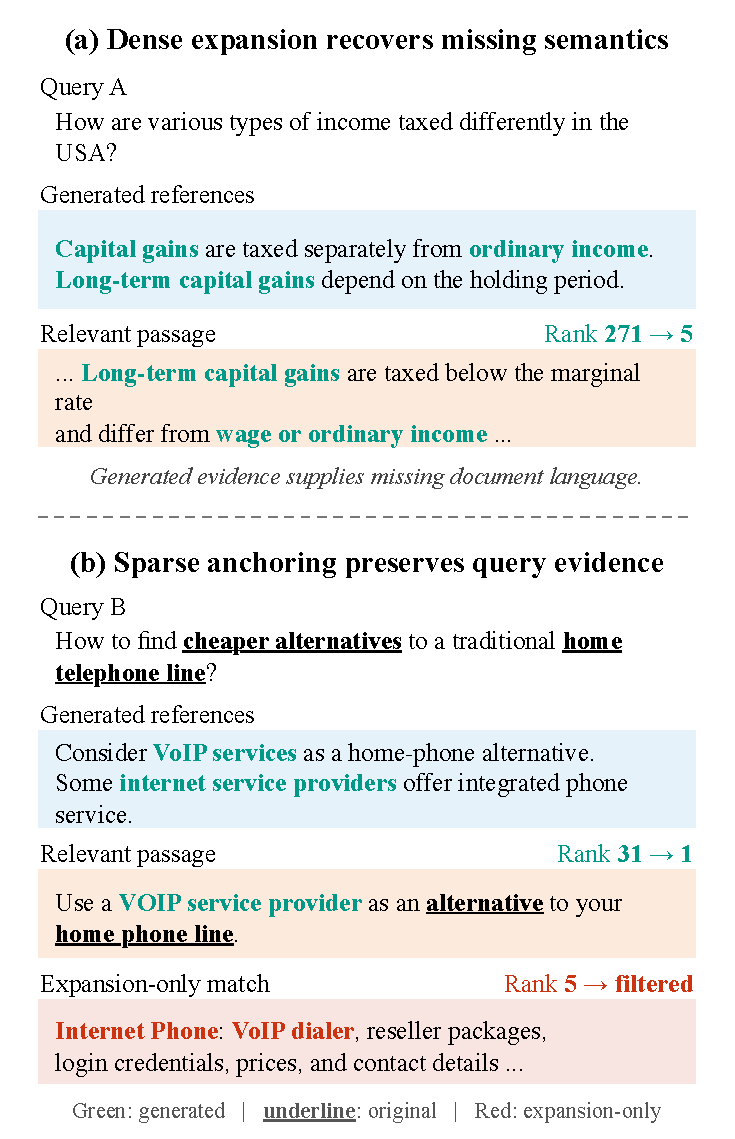
\includegraphics[width=\columnwidth]{figures/fig_desa_intuition.pdf}
  \caption{FiQA examples of DESA \citep{maia-etal-2018-fiqa, thakur-etal-2021-beir}. Dense expansion recovers missing document semantics; sparse anchoring promotes jointly supported passages and excludes expansion-only matches. Two references are shown per query; text is abridged and paraphrased, and ranks use draw~0.}
  \label{fig:desa-intuition}
\end{figure}

This evaluation view changes the design problem. The fused result and the depths required to certify it depend jointly on the dense and sparse rankings, so query construction for the two channels cannot be designed independently. Retriever-specific rewriting adapts each query to its own retriever, but does not explicitly control the cross-channel relation that governs exact fusion \citep{li-etal-2026-dvcqr}. We instead couple the two constructions through one shared set of generated references. Shared generation alone, however, is insufficient: applied directly to both channels, it enlarges sparse support on six of seven datasets, by as much as \(5.72\times\), and on NFCorpus reduces dense depth while increasing sparse depth. These observations motivate a coupled design that shares the evidence basis across channels but constrains its role within each channel.

DESA (Dense Expansion and Sparse Anchoring) implements this shared-generation, channel-specific-integration design. The LLM generates complementary reference passages once and supplies the same references to both channels. In dense retrieval, orthogonal residual expansion preserves the original query direction while adding the new semantic component supplied by the references. In sparse retrieval, score-product anchoring allows the references to reorder originally supported documents without introducing expansion-only matches. Together, these operators coordinate the two channels through shared evidence: dense retrieval can acquire new semantic support, while sparse retrieval remains anchored to the original query support (Figure~\ref{fig:desa-intuition}).

Across seven BEIR datasets, DESA improves equal-dataset macro nDCG@10 and Recall@20 over the unexpanded query by 3.82\% and 2.38\%, while reducing dense and sparse depths by 36.90\% and 36.56\%, respectively. With equal dataset weighting, 63.31\% of queries become shallower in both channels. Compared with matched Shared expansion, DESA significantly improves nDCG while preserving the original sparse support. Component analyses identify sparse anchoring as the more consistent source of effectiveness gains, with dense expansion providing complementary gains across most datasets.
